\documentclass[a4paper,12pt]{article}
\usepackage[utf8]{inputenc}
\usepackage[T1]{fontenc}
\usepackage[czech,english]{babel}
\usepackage{graphicx}
\usepackage{hyperref}
\usepackage{geometry}
\usepackage{xcolor}
\usepackage{float}
\geometry{margin=2.5cm}

\setlength{\parskip}{0.8em}
\setlength{\parindent}{0pt}

\begin{document}

\begin{center}
    {\Large \textbf{BPA-KOM Lab 1: Address Resolution Protocol (ARP)}}\\[1em]
\end{center}

\begin{center}
\begin{tabular}{|c|c|}
\hline
\textbf{Name} & Dave Galea \\ \hline
\textbf{VUT ID} & 284844 \\ \hline
\textbf{Lab Number} & 1 \\ \hline
\textbf{Date} & October 2025 \\ \hline
\end{tabular}
\end{center}

\vspace{0.5cm}
\hrule
\vspace{0.5cm}


\section*{1. Objective 1}

\textbf{Task Assignment:} \\
The aim of this task was to examine the ARP table on the local computer.

\vspace{0.5em}
\textbf{Solution:} \\
To view the ARP table, the command \texttt{arp -a} was used. Upon execution, this was the result:
\begin{figure}[H]
\centering
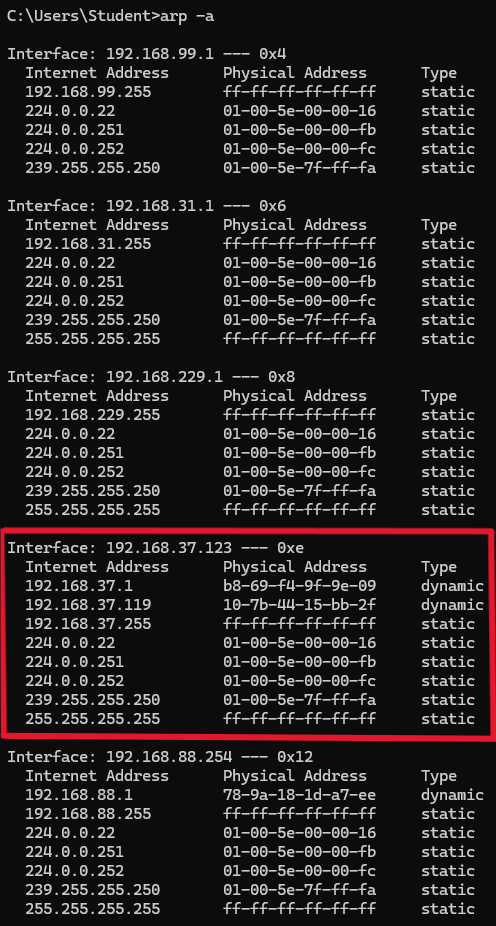
\includegraphics[width=\linewidth, height=0.55\textheight, keepaspectratio]{Pictures_Lab1/objective 1p1.png}
\caption{ARP table of the local computer.}
\end{figure}
Ethernet Adapter Public, identified through execution of the ipconfig command, is identified by IP 192.168.37.123 (the fourth interface). 
The presence of the dynamic record in the table is indicative that the computer has communicated with the router.

The static record with \textit{ff-ff-ff-ff-ff-ff} is used as a broadcast MAC address; it is used to send data to all devices on a local network.
\vspace{1em}
\hrule
\vspace{0.5em}

\section*{2. Objective 2}

\textbf{Task Assignment:} \\
The aim of this task was to capture and analyze the ARP communication between two computers in Wireshark.

\vspace{0.5 em}
\textbf{Solution:} \\
First, \texttt{ipconfig /all} was executed to give detailed information about the network configuration of the local devices.
\begin{figure}[H]
\centering
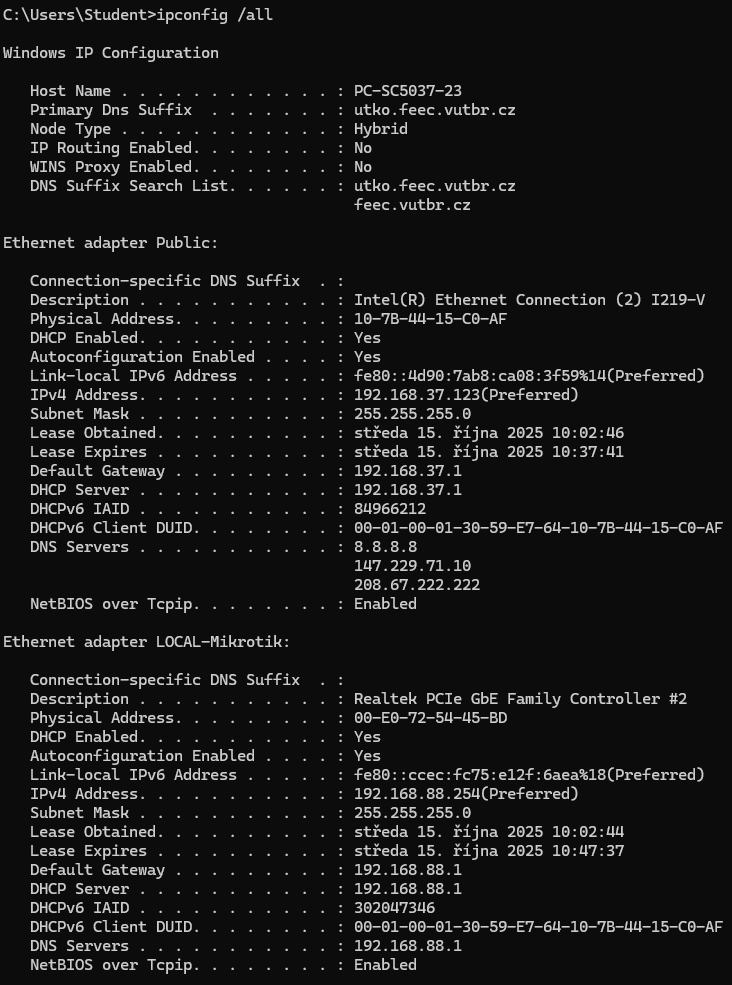
\includegraphics[width=\linewidth, height=0.55\textheight, keepaspectratio]{Pictures_Lab1/objective 2p1.png}
\caption{Output of ipconfig /all (first part).}
\end{figure}

\begin{figure}[H]
\centering
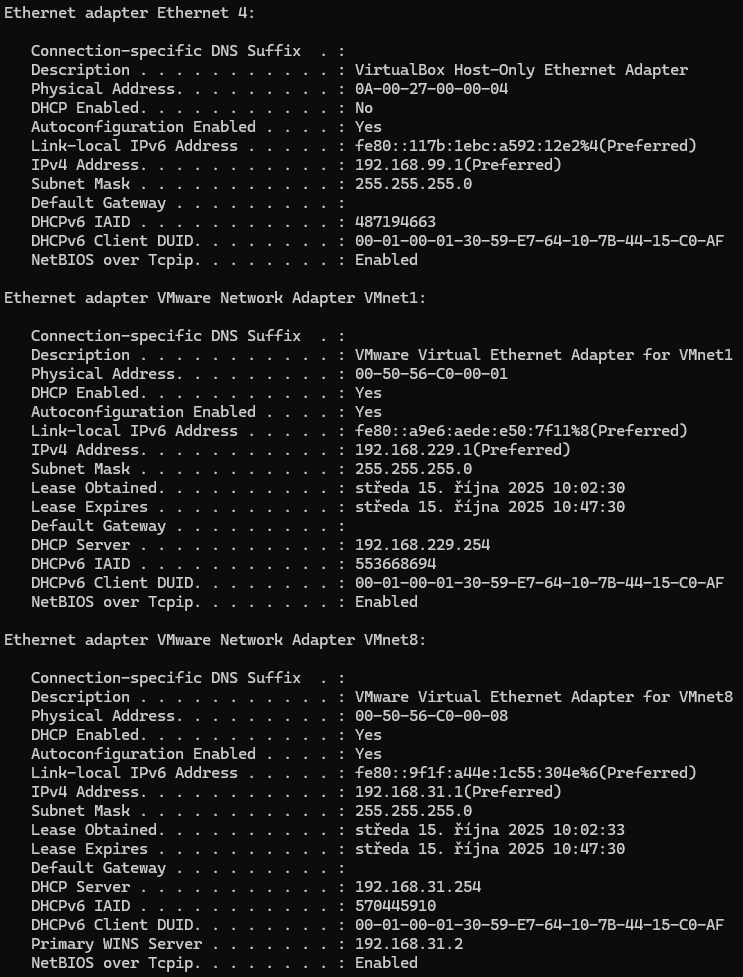
\includegraphics[width=\linewidth, height=0.55\textheight, keepaspectratio]{Pictures_Lab1/objective 2p2.png}
\caption{Output of ipconfig /all (continued).}
\end{figure}

The Ethernet interface of interest had the following:\\
\textit{IPv4 Address: }\texttt{192.168.37.123}\\
\textit{Physical Address: }\texttt{10-7B-44-15-C0-AF}

Then, in Wireshark, the arp filter was applied.
\begin{figure}[H]
\centering
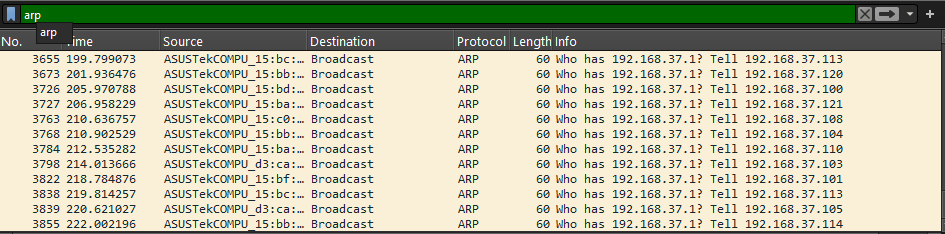
\includegraphics[width=\linewidth,keepaspectratio]{Pictures_Lab1/arp protocol applied.png}
\caption{Wireshark output after applying the arp protocol filter.}
\end{figure}

Then, one of two people generated an ARP request to obtain the MAC address of the other by using ping.
\begin{figure}[H]
\centering
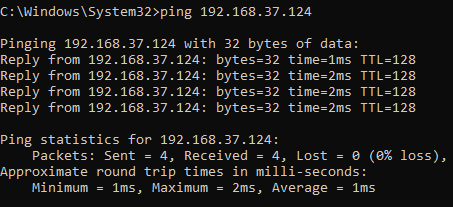
\includegraphics[width=\linewidth,keepaspectratio]{Pictures_Lab1/ping cmd.png}
\caption{Ping generated from the command line.}
\end{figure}

The result in Wireshark:
\begin{figure}[H]
\centering
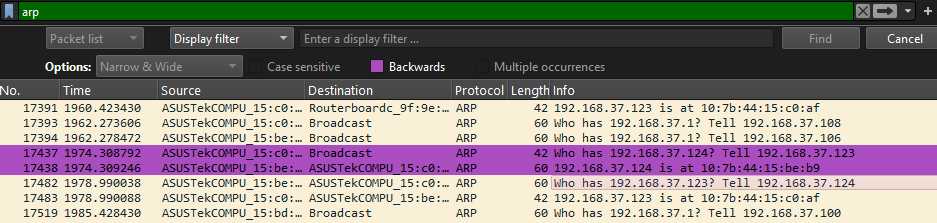
\includegraphics[width=\linewidth,keepaspectratio]{Pictures_Lab1/pinged.png}
\caption{The result of the ping displayed in Wireshark.}
\end{figure}


In the next section, both the ARP request packet and ARP response packet were examined.
\pagebreak

\textbf{ARP request} \\
Upon selecting the request packet details pane and expanding Ethernet II and Address Resolution Protocol:
\begin{figure}[H]
\centering
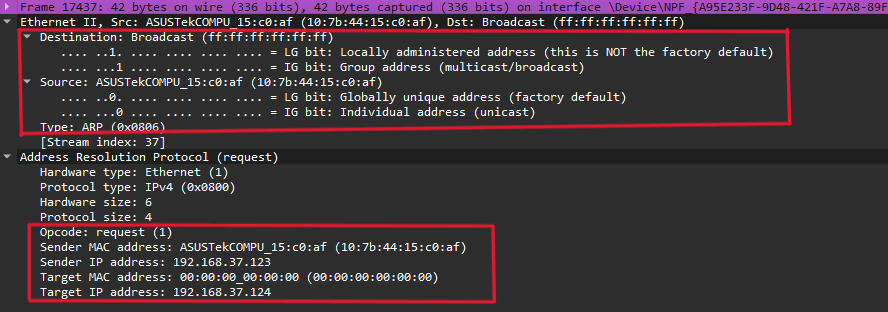
\includegraphics[width=\linewidth,keepaspectratio]{Pictures_Lab1/ethernet 2 and other thing ss .png}
\caption{Request packet details.}
\end{figure}
One can note that the Target MAC address, the address of who the data is intended for, is \texttt{00:00:00:00:00:00}; this is because it is still unknown; it will be known after the ARP response.
The Destination MAC address, the address of where the frame is physically meant to go, on the other hand, is \texttt{ff:ff:ff:ff:ff:ff}; because it is being broadcast to all devices on the LAN.
\vspace{1em}

\textbf{ARP Response} \\
Upon selecting the response packet details pane and expanding Ethernet II and Address Resolution Protocol:
\begin{figure}[H]
\centering
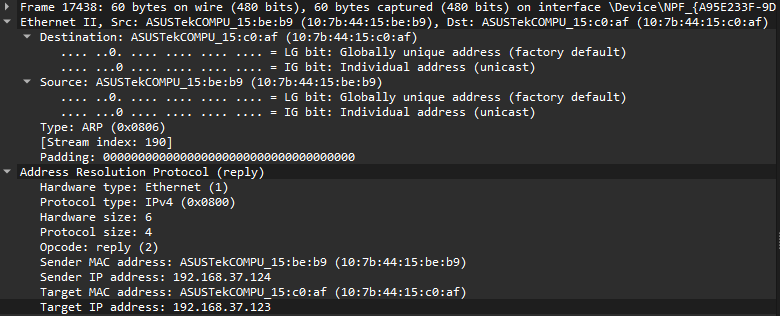
\includegraphics[width=\linewidth,keepaspectratio]{Pictures_Lab1/response packet answer ss.png}
\caption{Response packet details.}
\end{figure}

It can be noted that now, both the Target and Destination MAC addresses are the same, because the packet no longer needs to be flooded, and the packet can be sent directly.
\vspace{1em}
\hrule
\section*{3. Objective 3}
\textbf{Task Assignment:} \\
The aim of this task was to add the IP and MAC address of a colleague to the ARP table using the static method, and then examine the communication in Wireshark.

\textbf{Solution:} \\
The contents of the ARP table were re-displayed.
\begin{figure}[H]
\centering
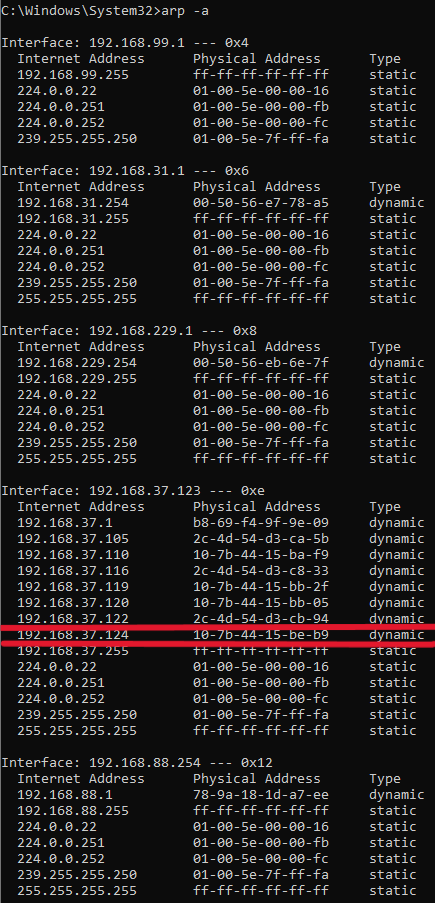
\includegraphics[width=\linewidth, height=0.55\textheight, keepaspectratio]{Pictures_Lab1/obj3 arp table .png}
\caption{Output of the redisplayed ARP table after previous actions.}
\end{figure}

The expected record; that of my colleague:
\begin{itemize}
    \item IP: \texttt{192.168.37.124}
    \item MAC: \texttt{10-7B-44-15-BE-B9}
\end{itemize}
was present in the table as a \textbf{dynamic} record.

Then, after removing the record using \texttt{arp -d <IP>}, the ARP table printed as follows:
\begin{figure}[H]
\centering
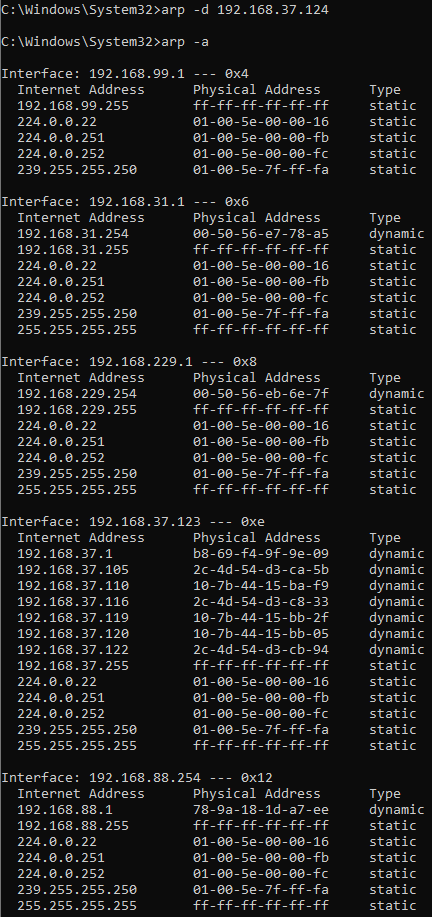
\includegraphics[width=\linewidth, height=0.55\textheight,  keepaspectratio]{Pictures_Lab1/arp-a after deletion obj3.png}
\caption{The ARP table after deleting the record.}
\end{figure}

It can be noted that my colleague's record is no longer present.

Then record was re-added manually.
This was done via \texttt{arp -s <IP> <MAC>}, with both IP and MAC being of my colleague. The result is a static record.

The \texttt{ping} command was then used to test the availability of my colleague.

\begin{figure}[H]
\centering
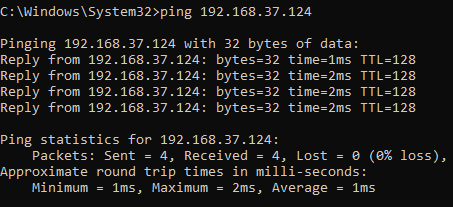
\includegraphics[width=\linewidth, height=0.16\textheight, keepaspectratio]{Pictures_Lab1/ping cmd.png}
\caption{The ping command executed in the command line.}
\end{figure}

After pinging, Wireshark was tested to see if any new ARP packets were captured. In theory, no new ARP packets should be captured, instead, the computer uses the pre-configured static mapping and bypasses the ARP process.
However, in our case, new packets were still captured as shown below. 
\begin{figure}[H]
\centering
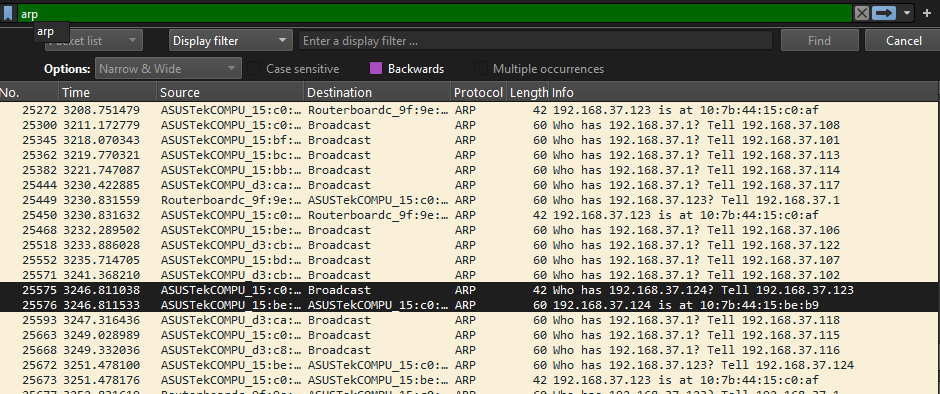
\includegraphics[width=\linewidth,keepaspectratio]{Pictures_Lab1/new arp generated anyway objective 3 .png}
\caption{Output in Wireshark after pinging.}
\end{figure}

\vspace{1em}
\hrule
\vspace{0.5em}
\pagebreak

\section*{4. Objective 4}

\textbf{Task Assignment:} \\
The aim of this task was to display the graph of captured packets in Wireshark.

\textbf{Solution:} \\
In Wireshark, captured packets can be displayed in a graph. After setting the filter to arp, setting the interval to 1 second, and measuring bytes, the following graph was produced:

\begin{figure}[H]
\centering
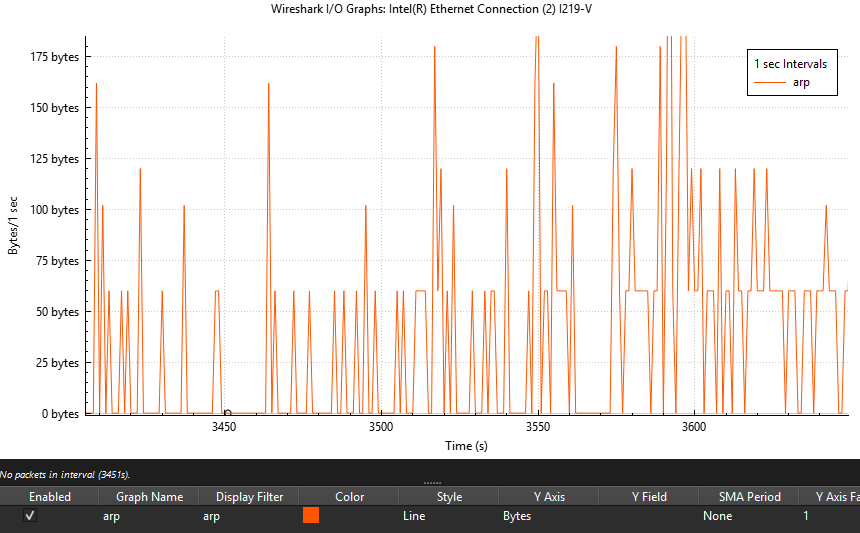
\includegraphics[width=\linewidth, keepaspectratio]{Pictures_Lab1/graph zoomed in.png}
\caption{Graph of Bytes captured over time.}
\end{figure}

It can be noted that many peaks are at 102 bytes; these represent the ARP request. The peaks are 102 bytes because as seen in wireshark; the length of the request packet is 60 bytes, and the length of the response packet is 42 bytes, making a total of 102 bytes in an ARP communication.

The graph can also be altered to display packets instead of bytes:
\begin{figure}[H]
\centering
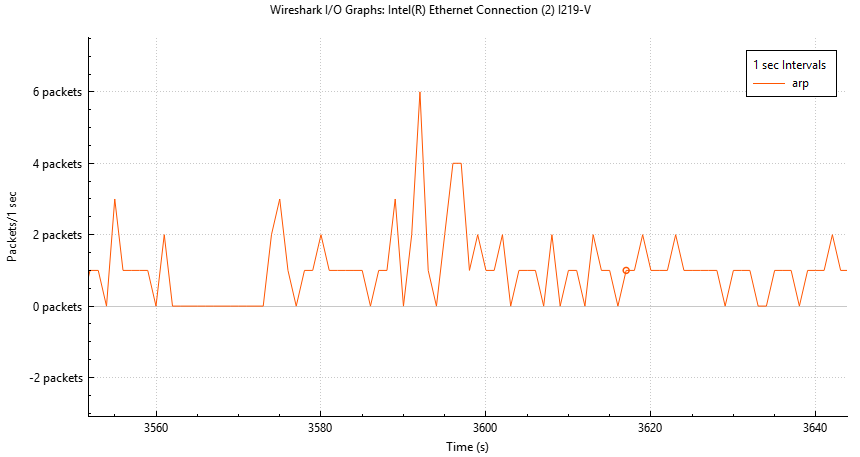
\includegraphics[width=\linewidth,keepaspectratio]{Pictures_Lab1/packets graph obj 4.png}
\caption{Graph of packets captured over time.}
\end{figure}
As confirmed by the bytes and the packets graphs, 2 packets are transferred per ARP communication.

\vspace{1em}
\hrule
\vspace{0.5em}
\pagebreak
\section*{5. Objective 5}

\textbf{Task Assignment:} \\
The aim of this task was to create a topology in Cisco Packet Tracer.

\textbf{Solution:} \\
To create the topology, the switch 2960 was connected via Copper Straight-Through cable to 4 PCs. The Fast Ethernet ports were used for connection.
\begin{figure}[H]
\centering
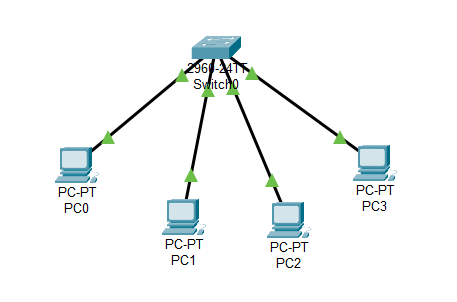
\includegraphics[width=\linewidth,keepaspectratio]{Pictures_Lab1/objective 5.png}
\caption{Topology created in Cisco Packet Tracer.}
\end{figure}

\vspace{1em}
\hrule
\vspace{0.5em}
\pagebreak
\section*{6. Objective 6}

\textbf{Task Assignment:} \\
The aim of this task was to generate and examine the ARP communication in a Packet Tracer Simulation. Additionally, the switch's MAC table was explored.

\textbf{Solution:} \\
After issuing the \texttt{ipconfig /all} command on each PC through the command prompt, the following table could be generated:
\begin{table}[H]
\centering
\begin{tabular}{|c|c|c|}
\hline
\textbf{Device} & \textbf{IP Address} & \textbf{MAC Address} \\ \hline
PC0 & 192.168.1.1 & 0060.3ECE.6DDC \\ \hline
PC1 & 192.168.1.2 & 00E0.F9A5.E89D \\ \hline
PC2 & 192.168.1.3 & 0002.17C3.D4E3 \\ \hline
PC3 & 192.168.1.4 & 000C.85AD.D769 \\ \hline
\end{tabular}
\caption{Device IP and MAC Address Table}
\end{table}

Then, Simulation Mode was enabled, and filters were applied to display ARP.
Before generating an ARP communication between PC0 and PC2, their respective ARP tables were checked to verify that they are empty.

From PC0, a ping was generated via \texttt{192.168.1.3}. This triggered a new event in the Event List, as shown below. 
\begin{figure}[H]
\centering
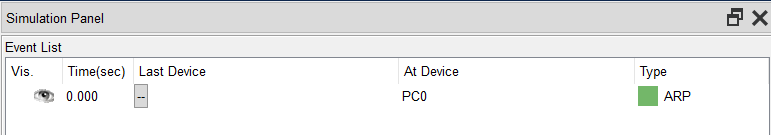
\includegraphics[width=\linewidth,keepaspectratio]{Pictures_Lab1/Event List obj 6 .png}
\caption{A new event displayed in the Event List.}
\end{figure}

Upon clicking this event, the OSI model is displayed, and it can be noted that only the lowest 2 layers contain data.
\begin{figure}[H]
\centering
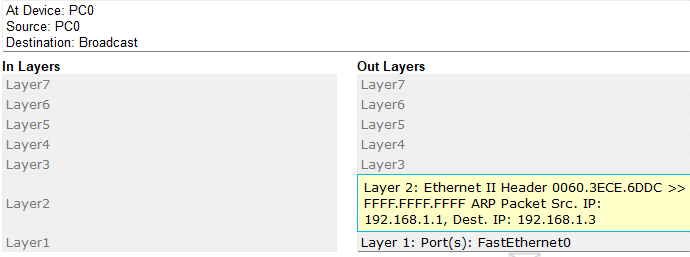
\includegraphics[width=\linewidth,keepaspectratio]{Pictures_Lab1/OSI obj 6 .png}
\caption{The OSI model displayed upon clicking the event.}
\end{figure}

Additionally, Outbound PDU details can be generated, as shown below.
\begin{figure}[H]
\centering
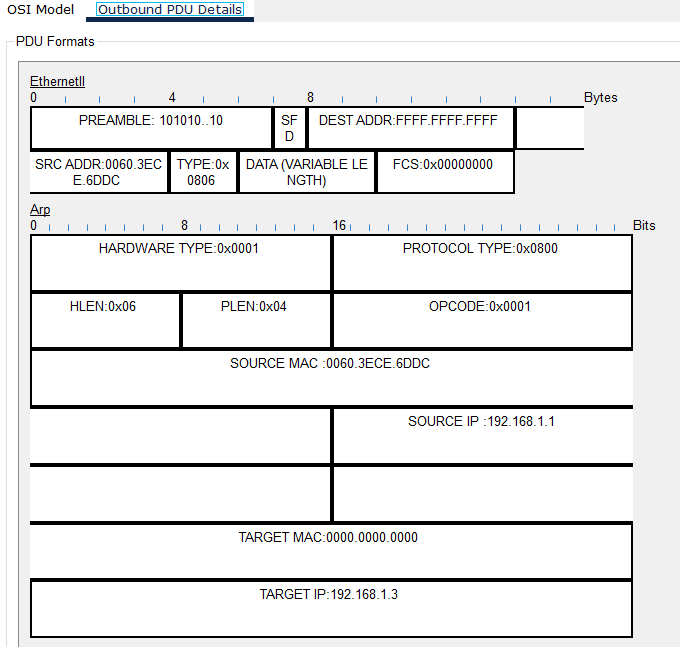
\includegraphics[width=\linewidth, height=0.55\textheight, keepaspectratio]{Pictures_Lab1/Outbound PDU details obj 6 .png}
\caption{The Outbound PDU details.}
\end{figure}
Important Details such as the source and target IP and MAC addresses, the destination MAC addresses, and the Opcode value can all be verified through this output.

The MAC address table of the switch can be observed through the CLI, using the command \texttt{show mac-address-table} while in \textbf{user mode}. In the lab it is expected that all PCs are already shown here; however, in my case, even after multiple attempts, the table showed empty, and only filled after the following steps.
\begin{figure}[H]
\centering
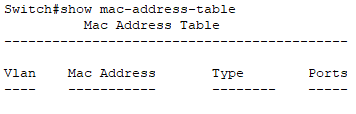
\includegraphics[width=\linewidth, height=0.15\textheight, keepaspectratio]{Pictures_Lab1/mac address obj6.7.png}
\caption{MAC address table observed through the CLI of the switch.}
\end{figure}

After Clicking Capture then forward, the frame arrives at the switch and the MAC table prints as follows:
\begin{figure}[H]
\centering
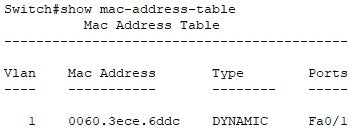
\includegraphics[width=\linewidth, height=0.15\textheight,keepaspectratio]{Pictures_Lab1/mac address obj6.8.png}
\caption{MAC address table after the frame arrives at the switch.}
\end{figure}

This is then repeated, and the frame is flooded out all ports except the inbound port. After clicking again, PC2 sends the packet to the switch. PC2's ARP table, at this stage, is as follows:
\begin{figure}[H]
\centering
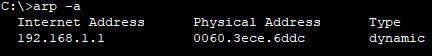
\includegraphics[width=\linewidth,keepaspectratio]{Pictures_Lab1/arp-a obj 6.10.png}
\caption{ARP table of PC2.}
\end{figure}
\pagebreak
The MAC table now has the following entries:
\begin{figure}[H]
\centering
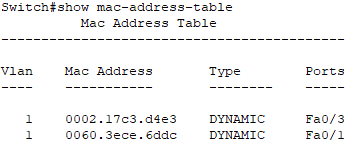
\includegraphics[width=\linewidth, height=0.15\textheight,keepaspectratio]{Pictures_Lab1/mac address obj6.10.png}
\caption{MAC address table after PC2 sends the packet to the switch.}
\end{figure}

And the Inbound PDU details are generated as follows:
\begin{figure}[H]
\centering
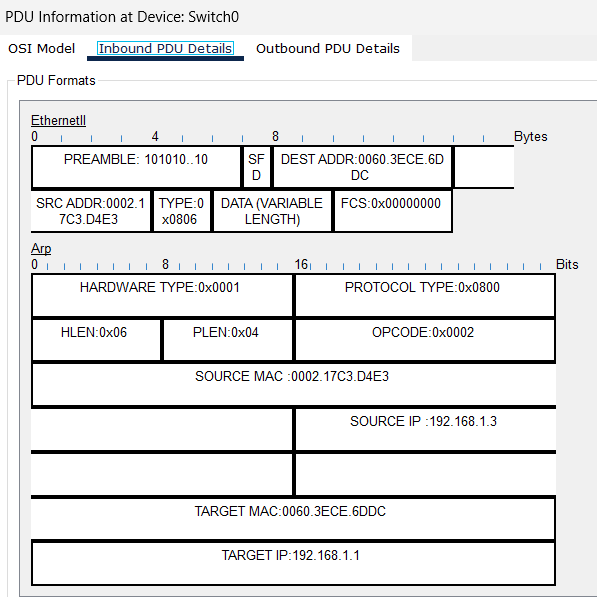
\includegraphics[width=\linewidth,keepaspectratio]{Pictures_Lab1/inbound pdu obj6.10.png}
\caption{Inbound PDU details.}
\end{figure}

Once again, important details such as the source and target IP and MAC addresses, the destination MAC addresses, and the Opcode value can all be verified through this output.//
For a final time, Capture then forward is pressed, and the switch sends the packet to PC0. The packet is not flooded, as the switch has the MAC addresses of the respective PCs, so flooding is unnecessary.

In the Command Prompt of PC0, the ICMP replies were successfully received, and the ARP table at PC0 is printed as follows:
\begin{figure}[H]
\centering
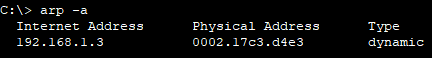
\includegraphics[width=\linewidth,keepaspectratio]{Pictures_Lab1/arp -a final .png}
\caption{ARP table at PC0 after the ARP communication is complete.}
\end{figure}

It can be noted that record in the ARP table at PC0 contains the address of PC2, meaning the ARP communication was successful

\vspace{1em}
\hrule
\vspace{0.5em}
\pagebreak

\section*{7. Final Questions}

\textbf{Question 1: What is the destination MAC address for the ARP request?} \\
The destination MAC address is the broadcast address \texttt{ff:ff:ff:ff:ff:ff}. This is because the ARP request is sent to all devices on the Local Area Network (LAN) since the requester does not yet know the MAC address of the target.

\textbf{Question 2: What is the Opcode (Operation) value for the ARP request and response?}\\
For the ARP request, the Opcode is 1, while for the ARP response, the Opcode is 2.

\textbf{Question 3: What values does the ARP table contain?} \\
The ARP table contains information about the values:
\begin{enumerate}
    \item IP Address of the device
    \item MAC Address of the device's network interface
    \item Type of entry (static or dynamic)
\end{enumerate}
\textbf{Question 4: What is the size of ARP packet?}\\
In this Lab, the request packet was 60 bytes, while the response packet was 42 bytes.

\textbf{Question 5: What is the difference between static and dynamic records in ARP table?} \\
Static records are manually configured, and while are rarely used, are useful for communicating with devices whose address does not vary over long periods; this is because static records have no timeout.\\
Dynamic records, on the other hand are automatically configured via ARP communication, and expire after a timeout of 2 minutes if not used, or a maximum of 10 minutes of continually used.

\textbf{Question 6: At which OSI layers does the ARP operate?} \\
ARP operates at the Data Link Layer and the Network Layer; it makes use of MAC address (a Data Link Layer address), and IP address (a Network Layer address)

\textbf{Question 7: What is the difference between ARP and MAC table?} \\
An ARP table contains mapping of IP addresses and MAC addresses of devices on the same local network, while a MAC table contains mapping of different device MAC addresses to a switch port.

\textbf{Question 8: What does the switch do with a packet whose destination address is not contained in the MAC table?}\\
The packet is flooded to all the ports except the port from which the packet came from. After flooding; the correct device responds, and it's MAC address is added to the MAC table for future reference.



\vspace{1em}
\hrule
\vspace{0.5em}

\end{document}
